% to choose your degree
% please un-comment just one of the following
\documentclass[bsc,logo,frontabs,twoside,singlespacing,normalheadings,parskip]{infthesis}     % for BSc, BEng etc.
% \documentclass[minf,frontabs,twoside,singlespacing,parskip]{infthesis}  % for MInf


% FONT COMMANDS
\usepackage{fontspec}
\setmainfont[Mapping=tex-text,Numbers=OldStyle]{fbb}
\setsansfont[Mapping=tex-text,Numbers=OldStyle,Scale=MatchLowercase]{Gill Sans}
\setmonofont[Mapping=tex-text,Scale=MatchLowercase]{Inconsolata}


% DISPLAY TODOS
%\usepackage[disable]{todonotes}
\usepackage[draft,bordercolor=white,backgroundcolor=yellow!60,linecolor=black,colorinlistoftodos]{todonotes}


% MAKE SURE TODOS ARE INLINE
\let\Oldtodo\todo
\renewcommand{\todo}[1]{\Oldtodo[inline]{#1}}

% INCLUDE CODE FILES
\usepackage{minted}

% ALLOW TWO FIGURES NEXT TO EACH OTHER
\usepackage{subcaption}


% ENSURE CHAPTERS WORK IN PDF VIEWERS
\usepackage[]{hyperref}
\hypersetup{
    pdftitle={Storm on Multi-core},
    pdfauthor={Mark Nemec},
    %pdfsubject={Your subject here},
    %pdfkeywords={keyword1, keyword2},
    bookmarksnumbered=true,
    bookmarksopen=true,
    bookmarksopenlevel=1,
    %colorlinks=true,
    pdfstartview=Fit,
    pdfpagemode=UseOutlines,
    pdfpagelayout=TwoPageRight
}

\begin{document}

\title{Storm on Multi-core}

\author{Mark Nemec}

% to choose your course
% please un-comment just one of the following
% \course{Artificial Intelligence and Computer Science}
%\course{Artificial Intelligence and Software Engineering}
%\course{Artificial Intelligence and Mathematics}
%\course{Artificial Intelligence and Psychology }
%\course{Artificial Intelligence with Psychology }
%\course{Linguistics and Artificial Intelligence}
\course{Computer Science}
%\course{Software Engineering}
%\course{Computer Science and Electronics}
%\course{Electronics and Software Engineering}
%\course{Computer Science and Management Science}
%\course{Computer Science and Mathematics}
%\course{Computer Science and Physics}
%\course{Computer Science and Statistics}

% to choose your report type
% please un-comment just one of the following
%\project{Undergraduate Dissertation} % CS&E, E&SE, AI&L
%\project{Undergraduate Thesis} % AI%Psy
\project{4th Year Project Report}

\date{\today}

\abstract{
This is an example of {\tt infthesis} style.
The file {\tt skeleton.tex} generates this document and can be
used to get a ``skeleton'' for your thesis.
The abstract should summarise your report and fit in the space on the
first page.
%
You may, of course, use any other software to write your report,
as long as you follow the same style. That means: producing a title
page as given here, and including a table of contents and bibliography.
}

\maketitle

\section*{Acknowledgements}
Acknowledgements go here.

\tableofcontents

\pagenumbering{arabic}


%%%%%%%%%%%%%%%%%%%%%%%%%%%%%%%%%%%%%%%%%%%%%
%%
%%				INTRODUCTION
%%
%%%%%%%%%%%%%%%%%%%%%%%%%%%%%%%%%%%%%%%%%%%%%


\chapter{Introduction}

In recent years, there has been an explosion of cloud computing software. After Google published their paper on MapReduce \cite{Anonymous:Jj3E6x7v}, many new open-source frameworks for distributed computation have emerged, most notably Apache Hadoop for batch processing and Apache Storm for real-time data stream processing.

The main idea of these frameworks is to split the work that needs to be carried out and distribute it across multiple nodes of a cluster. Commercial companies and researchers have been able to utilise these frameworks and create distributed systems \cite{5billion-sessions} which can accomplish things that would not be possible on a single computer. This has mostly been allowed by the low price of commodity hardware and good horizontal scaling properties.

% TODO: Here talk about What this paper is about !
% TODO: Maybe mention the Hadoop multi-core paper
% TODO: Maybe a section - move main idea here?
This project is about taking the ideas from the distributed system Apache Storm and applying them in the context of multi-core machines instead of clusters.

%% TODO: After that comes Motivation which explains why it's a good idea!
\section{Motivation}

While the cost of a commodity hardware cluster might be lower than the price of a single computer with equal power there are certain limitations:

\begin{itemize}

\item The nodes of a cluster communicate through network. This limits the speed of communication between processes that live on different nodes.

\item Distributed systems waste resources by replicating data to ensure reliability.

% TODO: Maybe mention renting vs owning here
\item Running a distributed computation on commodity hardware usually requires a data centre or renting out instances on cloud computing services such as Amazon EC2 or Rackspace. This is not ideal for some use cases which require full control over the system or a heightened level of security. 

\end{itemize}

On the other hand, even though Moore’s law still holds true, processor makers now favour increasing the number of cores in CPU chips to increasing their frequency. This trend implies that the “free lunch” of getting better software performance by upgrading the processor is over and programmers now have to design systems with parallel architectures in mind. However, there are some limitations to this as well:

\begin{itemize}

\item It is generally believed that writing parallel software is hard. The traditional techniques of message passing and parallel threads sharing memory require the programmer to manage the concurrency at a fairly low level, either by using messages or locks.

%% TODO: Rephrase "nice if they could"
\item Apache Storm has become the de facto tool used in stream processing on a cluster and according to their "Powered By" page \cite{Anonymous:eikzOt4-} there are tens of companies already using Storm to process their real-time streams. It would be nice if they could keep that code.

\end{itemize}

\section{Main Idea}

The solution proposed in this paper is to take the existing Apache Storm project and port it for multi-core machines. This is implemented in a library Storm-MC with an API compatible with Apache Storm. This allows us to take an existing application written with Apache Storm in mind and run it in a multi-core setting. This way, we can avoid network latency and enjoy the significant performance improvements of a shared-memory environment.

\begin{itemize}

	\item Prices of high-end server have decreased and one can get a 32-core machine for 10,000 USD.

\end{itemize}

\section{Structure of the Report}
%% And after that explain the structure of the report :)

In chapter 1, blah blah.


%%%%%%%%%%%%%%%%%%%%%%%%%%%%%%%%%%%%%%%%%%%%%
%%
%%				BACKGROUND
%%
%%%%%%%%%%%%%%%%%%%%%%%%%%%%%%%%%%%%%%%%%%%%%


\chapter{Background}

In this chapter we give background information necessary to understand the design of Storm-MC. Apache Storm is developed in a mix of Java and Clojure. As mentioned by the author of Storm in \cite{Marz_2014}, writing the Storm interfaces in Java ensured large potential user-base while writing the implementation in Clojure increased productivity.

To ensure API compatibility with Storm, Storm-MC was developed using the same languages. This allowed for great code reuse and not getting slowed down by re-implementing functionality already present in Storm in a different language.

\section{Core Concepts}

There are several core concepts used by Storm and hence by extension Storm-MC as well. These concepts are put together to form a simple API that allows the user to break down a computation into separate components and define how these components interact with each other. The three core concepts of Storm are:

\begin{description}
  \item[Spout] \hfill \\
  A spout is a component that represents the source of a data-stream. Typically, a spout reads from a message broker such as RabbitMQ \cite{RabbitMQ} or Apache Kafka \cite{ApacheKafka} but can also generate its own stream or read from somewhere like the Twitter streaming API.
  \item[Bolt] \hfill \\
  A bolt is a component that transforms tuples from its input data stream and emits them to its output data stream. A bolt can perform a range of functions e.g. filter out tuples based on some criteria or perform a join of two different input streams.
  \item[Topology] \hfill \\
  The programmer connects spouts and bolts in a directed graph called topology which describes how the components interact with each other. The topology is then submitted to Storm for execution.
\end{description}

\section{Example Topology}

\begin{figure}[!htb]
	\centering
	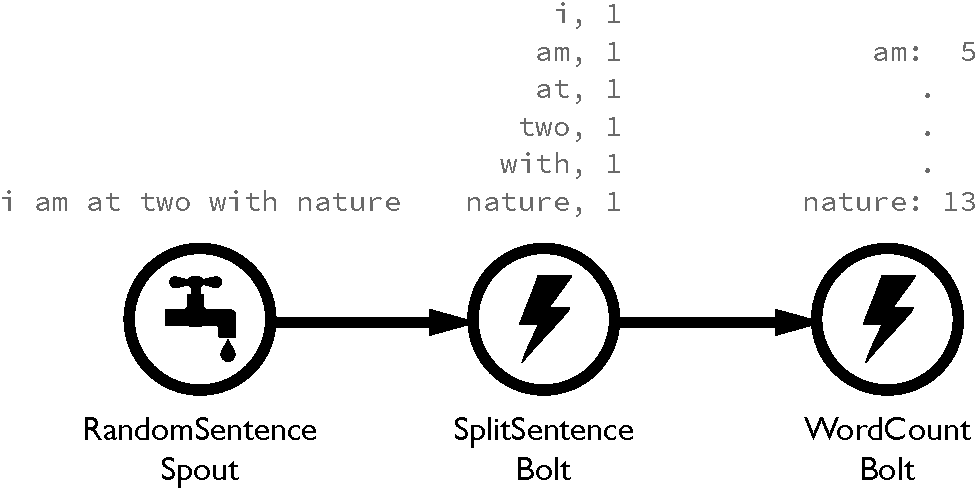
\includegraphics[scale=0.7]{pdf/wordcount_topology.pdf}
	\caption{WordCount topology.}
	\label{fig:wordcount_topology}
\end{figure}

A classic example used to explain Storm topologies is the WordCount topology. In this topology, there is a spout generating random sentences, a bolt splitting the sentences on white space, and a bolt counting occurrences of every word. Figure \ref{fig:wordcount_topology} shows how we could represent this topology graphically.

This may seem as a simplistic example but it is useful when demonstrating how easy it is to implement a working topology using the Storm API.

\begin{listing}[!htb]
\inputminted{java}{code/WordCountTopology.java}
\caption{WordCountTopology.java}
\label{listing:wordcount_topology}
\end{listing}

Listing \ref{listing:wordcount_topology} shows how the topology is put together to form a graph of components. Storm uses the Builder design pattern to build up the topology which is then submitted to Storm for execution. The last argument to the setBolt/setSpout method is the number of parallel tasks we want Storm to execute for the respective component.

\newpage

\begin{listing}[!htb]
\inputminted{java}{code/RandomSentenceSpout.java}
\caption{RandomSentenceSpout.java}
\label{listing:wordcount_spout}
\end{listing}

Listing \ref{listing:wordcount_spout} shows the definition of a spout that emits a randomly chosen sentence from a predefined collection of sentences.

\newpage

\begin{listing}[!htb]
\inputminted{java}{code/SplitSentence.java}
\caption{SplitSentence.java}
\label{listing:wordcount_split}
\end{listing}

\begin{listing}[!htb]
\inputminted{python}{code/splitsentence.py}
\caption{splitsentence.py}
\label{listing:wordcount_split_py}
\end{listing}

Listings \ref{listing:wordcount_split} and \ref{listing:wordcount_split_py} show how a bolt defined in Python can be part of this Java-defined topology.

\newpage

\begin{listing}[!htb]
\inputminted{java}{code/WordCount.java}
\caption{WordCount.java}
\label{listing:wordcount_count}
\end{listing}

Finally, listing \ref{listing:wordcount_count} shows how a bolt that counts the number of word occurrences can be implemented.


\section{Additional Concepts}

\begin{description}
  \item[Stream] \hfill \\
  A stream is defined as an unbounded sequence of tuples. Streams can be thought of as edges of a topology connecting bolts and spouts (vertices).
  \item[Tuple] \hfill \\
  A tuple wraps named fields and their values. The values of fields can be of different types. When a component emits a tuple to a stream it sends that tuple to every bolt subscribed to the stream.
  \item[Stream Grouping] \hfill \\
  Every bolt needs to have a type of stream grouping associated with it. This grouping decides the means of distributing the tuples coming from the bolt's input streams amongst the instances of the bolt task. Following are the possible types of stream grouping:
  \begin{description}
  	\item[Shuffle] Randomly partitions the tuples among all the bolt tasks.
  	\item[Fields] Hashes on a subset of the tuple fields.
  	\item[All] Replicates the entire stream to all the bolt tasks.
  	\item[Direct] The producer of the tuple decides which task of the bolt will receive this tuple.
  	\item[Global] Sends the entire stream to a single bolt task.
  	\item[Local or Shuffle] Prefers sending to executors in the same worker process, if that is not possible it uses the same strategy as shuffle.
  \end{description}
\end{description}

Users are also able to specify their own custom grouping by implementing the \texttt{CustomStreamGrouping} interface.

\todo{Explain why you would want to do that.}

All the components of a Storm topology execute in parallel. The user can specify how much parallelism he wants associated with every component and Storm spawns the necessary number of threads. This is done through a configuration file, defined in YAML, which is submitted along with the topology.

\todo{talk more about config}

\section{Storm Architecture}

\begin{figure}[!htb]
	\centering
	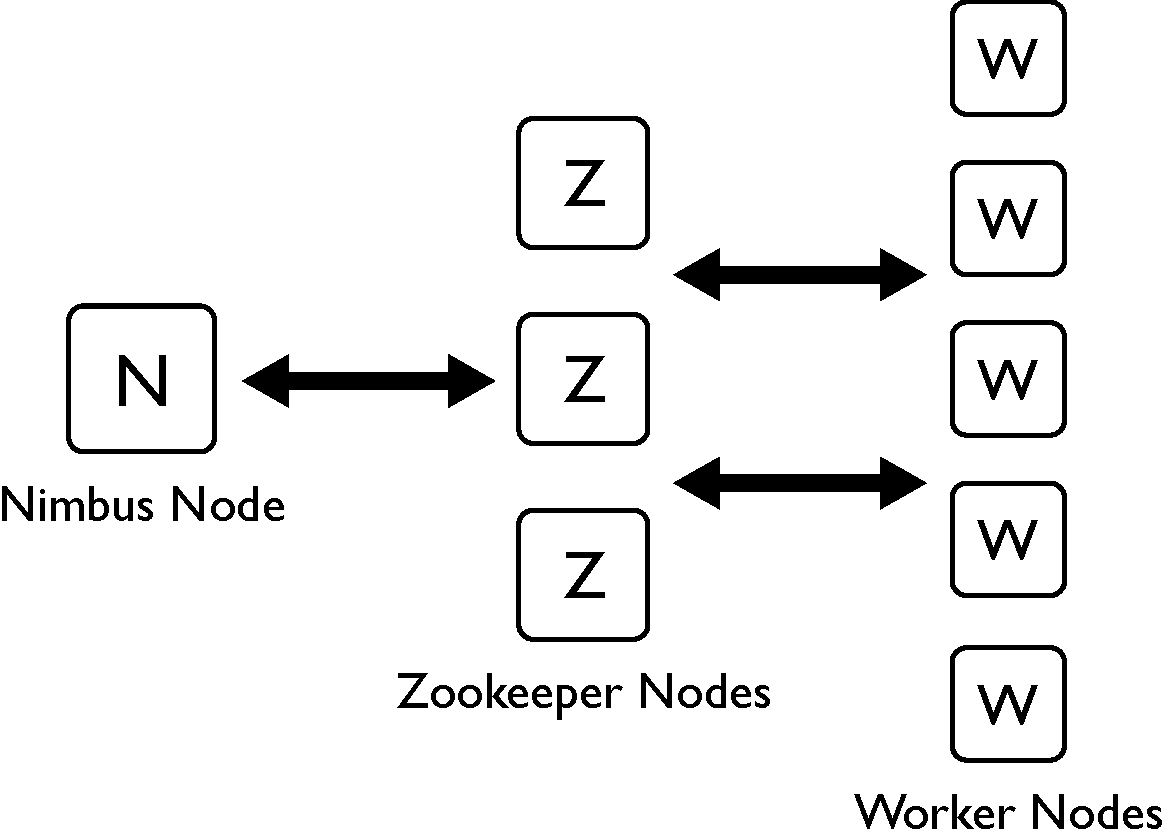
\includegraphics[scale=0.5]{pdf/storm_arch.pdf}
	\caption{Apache Storm Architecture.}
	\label{fig:storm_arch}
\end{figure}

\todo{Maybe highlight similarities to Hadoop}

A Storm cluster adopts the Master-Worker pattern. To set up a Storm topology, the user launches daemon processes on nodes of the cluster and submits the topology to the master node, also called Nimbus. The worker nodes receive task assignments from the master and execute on them. The coordination between the master node and the worker nodes is handled by nodes running Apache Zookeeper \cite{ApacheZookeeper}. Figure \ref{fig:storm_arch} shows a graphical representation of Storm Architecture.

\subsection{Nimbus Node}

The master node runs a server daemon called Nimbus. The main role of Nimbus is to receive topology submissions from clients. Upon receiving a topology submission, Nimbus takes the following steps:

\begin{description}
	\item[Validate the topology] \hfill \\
	The topology is validated using a validator to ensure that the submitted topology is valid before trying to execute it. The user can implement his own validator or use the default validator provided by Storm.
	\item[Distribute the topology source code] \hfill \\
	Nimbus ensures that the workers involved in the topology computation have the source code by sending it over the network.
	\item[Schedule the topology] \hfill \\
	Nimbus runs a scheduler that distributes the work among workers of the cluster. Similarly to validation, the user can implement his own scheduler or use the default scheduler provided by Storm. The default scheduler uses a simple Round-robin strategy.
	\item[Activate the topology] \hfill \\
	Nimbus transitions the topology to active state which tells the worker nodes to start executing it.
	\item[Monitor the topology] \hfill \\
	Nimbus continues to monitor the topology by reading heartbeats sent by the worker nodes to ensure that the topology is executing as expected and worker nodes have not failed.
\end{description}


Nimbus is an Apache Thrift \cite{ApacheThrift} service (more on Thrift in section \ref{sec:serialisation}) that listens to commands submitted by clients and modifies the state of a cluster accordingly. Following are the commands supported by Nimbus:

\begin{description}
	\item[Submit a topology] \hfill \\
	Clients can submit a topology defined in a Java Archive (JAR) file. The Nimbus service then ensures that the topology configuration and resources are distributed across the cluster and starts executing the topology.
	\item[Kill a topology] \hfill \\
	Nimbus can stop running a topology and remove it from the cluster. The cluster can still continue executing other topologies.
	\item[Activate/deactivate a topology] \hfill \\
	Topologies can be deactivated and reactivated by Nimbus. This could be useful if the spout temporarily cannot produce a stream and the user does not want the cluster to execute idly.
	\item[Rebalance a topology] \hfill \\
	Nimbus can rebalance a topology across more nodes. Thus if the number of nodes in the cluster changes the user can increase or decrease the number of nodes involved in the topology.
\end{description}

%\todo{Is listing this really necessary?}

\subsection{Worker Nodes}

The worker nodes run a daemon called Supervisor. There are 4 layers of abstraction which control the parallelism of a worker node.

\begin{description}
	\item[Supervisor] \hfill \\
	A supervisor is a daemon process the user runs on a worker node to make it part of the cluster. It launches worker processes and assigns them a port they can receive messages on. Furthermore, it monitors the worker processes and restarts them if they fail. A worker node runs only one supervisor process.
	\item[Worker] \hfill \\
	A worker process is assigned a port and listens to tuple messages on a socket associated with the port. A worker launches executor threads as required by the topology. Whenever it receives a tuple, it puts it on a queue where it is picked up by one or more executors of the worker process.
	
	Furthermore, the worker has a transfer queue where its executors enqueue tuples ready to be sent downstream. There can be multiple workers processes running inside one supervisor.
	\item[Executor] \hfill \\
	An executor controls the parallelism within a worker process. Every executor runs in a separate thread. An executor's job is to pick up tuples from the receiver queue of the worker, perform the task of a component it represents, and put the transformed tuples on the transfer queue of the worker. There can be many executors running inside one worker and an executor performs one (the usual case) or more tasks.
	\item[Task] \hfill \\
	A task represents the actual tuple processing function. However, within an executor thread all the tasks are executed sequentially. The main reason for having tasks is that the number of tasks stays the same throughout the lifetime of a topology but the number of executors can change (by rebalancing). Thus if some worker nodes in the cluster go down, the topology can continue executing with the same number of tasks as before.
\end{description}

\subsection{Zookeeper Nodes}

The Storm cluster contains a number of Zookeeper nodes which coordinate the communication between the master and the workers. Storm does this by storing the state of the cluster on the Zookeper nodes where both Nimbus and worker nodes can access it.

The cluster state contains worker assignments, information about topologies, and heartbeats sent by the worker nodes back to Nimbus. Apart from the cluster state, Storm is completely stateless. Hence, if the master node or a worker node fail the cluster continues executing. The only time the cluster stops executing is if all the Zookeper nodes die.

\section{Tuple Processing}
\label{sec:tuple_processing}

\begin{figure}[!htb]
	\centering
	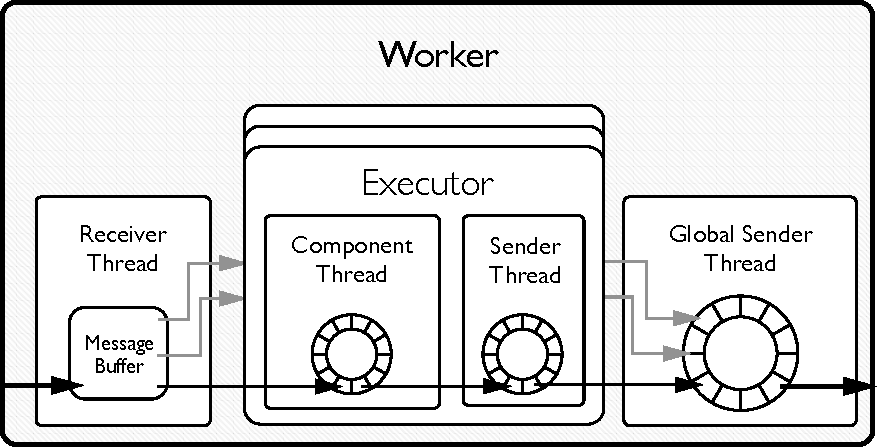
\includegraphics[scale=0.7]{pdf/worker_inside.pdf}
	\caption{Tuple processing in Apache Storm.}
	\label{fig:worker_inside}
\end{figure}

Figure \ref{fig:worker_inside} shows how tuple processing is implemented inside a Storm worker process. The tuple is read from a message buffer by the receiver thread of the worker and put on a corresponding executor's receiver queue. The tuple is then picked up by the component thread of an executor.

After the component thread has executed the task it puts the tuple on the sender queue. There, it is picked up by the executor's sender thread which puts the tuple on the global sender queue of the worker. Lastly, the global sender thread of the worker serialises the tuple and sends it downstream.

Alternatively, if the tuple is forwarded to an executor in the same worker process it is put on the receiver queue of the corresponding executor directly after processing.

Storm uses the term queue freely but in fact the queues are implemented as ring buffers using LMAX Disruptor \cite{LMAX_Disruptor}. Detailed background of how Disruptor works and its performance benchmarks can be found in \cite{Thompson_Farley_Barker_Gee_Stewart_2011}.

\section{Serialisation}
\label{sec:serialisation}

Since Storm topologies execute on a cluster all the components need to be serialisable. This is achieved with Apache Thrift. Components are defined as Thrift objects and Thrift generates all the Java serialisation code automatically.

\todo{Why is Thrift good?}

Furthermore, since Nimbus is a Thrift service Thrift generates all the code required for remote procedure call (RPC) support. This allows defining topologies in any of the languages supported by Thrift and easy cross-language communication with the Nimbus service.


%%%%%%%%%%%%%%%%%%%%%%%%%%%%%%%%%%%%%%%%%%%%%
%%
%%				   DESIGN
%%
%%%%%%%%%%%%%%%%%%%%%%%%%%%%%%%%%%%%%%%%%%%%%


\chapter{Bringing Storm to Multi-core}

% - Explain why original Storm is bad
% - Explain high-level
% - Explain Nimbus - assignments are useless though
% - Explain how executors interact within a worker - messages


The design of Storm-MC was ported over from Apache Storm. This enabled rapid progress while guaranteeing compatibility with Apache Storm API. Clearly, however, some differences had to be made to take advantage of multi-core machine performance implications. This chapter explains the design of Storm-MC.

\section{Apache Storm on Multi-core}

To begin, we discuss why Apache Storm does not perform optimally on a single multi-core machine. Storm can be ran in local mode where it emulates execution on a cluster. This mode exists so that it is possible to debug and develop topologies without needing access to a cluster. However, there are several reasons why the local mode is not as performant as it could be.

We described tuple processing in Storm in section \ref{sec:tuple_processing}. Clearly, there is a lot of overhead necessary to simulate sending tuples to executors in other worker nodes. This overhead comes not only from the tuple passing through several queues but also includes running a Netty \cite{Netty} server used for message passing.

Storm runs many threads which are only useful in distributed context. Indeed, during our experiments we found that a topology with 8 executors was being executed with 64 threads.

\todo{Plot threads vs components}
\todo{Maybe include Thread Dump and a graph of thread counts}

Additionally, every worker has a heartbeat thread that simulates sending heartbeat messages to the Nimbus process. It does this by writing to a local cache which is persisted to a file by a blocking write on every heartbeat. While heartbeats are essential in cluster mode, there is no need for them in local mode.

Another overhead is running a local Zookeper server which emulates the Zookeeper nodes of a cluster. State is maintained in this server even though there is always only one topology executing at a time.

%	\item[Fault Tolerance] \hfill \\
%	Storm is made to be fault-tolerant. This means that it can guarantee a tuple being processed from its spout all the way to its final bolt. To do this it adds an additional acker bolt to every topology. This bolt acts as a root of a tree with the nodes being all the components the tuple "goes" through. If the tuple gets successfully processed by a component its node is marked as "acked". Hence once all nodes of the tree are marked as "acked" Storm can guarantee the tuple was processed.
%	\item[Redundant threads] \hfill \\
%	Storm runs many threads which are only useful in distributed context. Indeed, during our experiments we found that a topology with 8 executors was being executed with 64 threads. This included threads which were used as timeout timers or to send heartbeats and were unnecessary in a multi-core setting. Obviously, not all of them were executing in parallel but there is clearly room for reduction.

\section{Storm-MC Architecture}

\todo{Probably don't call this Architecture}

The design we adopted for porting worker nodes is to only have one worker process running all the executor threads of a topology.

Additionally, the code for the Nimbus daemon was merged with the worker. This was done because there is no need to run the Nimbus and worker specific code at the same time. Once Nimbus sets up the topology, all the work is done by the worker. Hence they can be executed serially.

\subsection{Nimbus}

Unlike Nimbus executing on a Storm cluster, Nimbus in Storm-MC does not support running multiple topologies at the same time. However, to do that one only needs to run the topology in a separate process. This is because unlike when executing on the cluster different topologies do not need to share any state and it is more natural to execute them as separate processes.

This has the added benefit of each process having its own part of main memory thus reducing cache conflicts as shown in \cite{Chandra:2005:PIC:1042442.1043432} and providing higher security by not having different topologies share memory space. Additionally, if a single thread of one topology is blocking it does not block other topologies.

Nimbus on Storm-MC does not support scheduling topologies. Since within one process there is only one topology running at a time and the hardware configuration of the machine does not change, the parallelism is clearly defined by the number of executors per component specified in the topology configuration.

One way to implement scheduling could be to pin threads to specific cores. Unfortunately, Java does not provide support for CPU affinity, the assignments are handled automatically by the JVM. Potentially, this could be achieved by using C or C++, both of which support CPPU affinity, but this was not implemented in Storm-MC.

\todo{Mention porting over from Thrift.}

The role of Nimbus in Storm-MC has effectively been reduced to validating the topology and passing it along to the worker part of the process which handles the topology execution.

\subsection{Worker}

In Apache Storm, a worker node runs the supervisor daemon, which in turns launches worker processes which contain executor threads which contain tasks. In Storm-MC, however, there is only one worker process which contains all the executor threads and their tasks.

This design has several benefits:

\begin{itemize}
	\item All the inter-thread communication is occurring within one Worker.
	\item Supervisor can be removed as there is no need to synchronise workers.
	\item There is no need to simulate over-the-network message passing.
	\item Message passing between executor threads within a worker stays the same as in Apache Storm.
\end{itemize}

A comparison of an Apache Storm worker node and its Storm-MC equivalent can be seen in figure \ref{fig:comparison}.

\begin{figure}[!htb]
\centering
\begin{subfigure}{.5\textwidth}
  \centering
  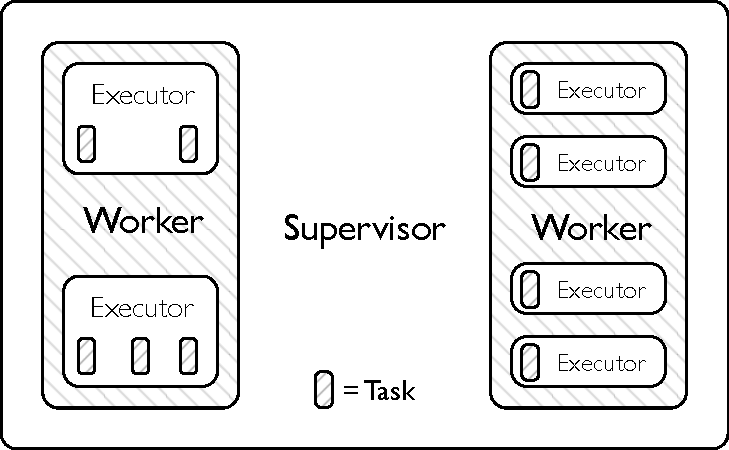
\includegraphics[width=0.95\linewidth]{pdf/distributed_worker.pdf}
  \caption{Worker in Apache Storm.}
  \label{fig:comparison1}
\end{subfigure}%
\begin{subfigure}{.5\textwidth}
  \centering
  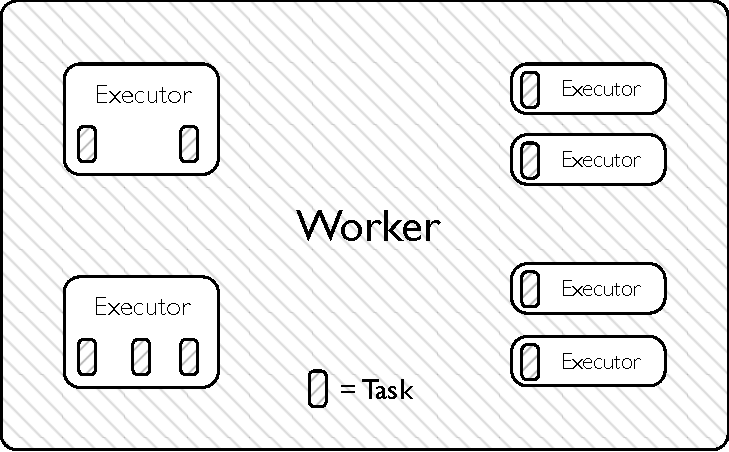
\includegraphics[width=0.95\linewidth]{pdf/local_worker.pdf}
  \caption{Worker in Storm-MC.}
  \label{fig:comparison2}
\end{subfigure}
\caption{Comparison of a worker in Storm and Storm-MC}
\label{fig:comparison}
\end{figure}

\subsection{State}

In light of previous subsections Storm-MC is completely stateless. The cluster state that was managed by Zookeeper in Apache Storm was completely stripped away. This state was only relevant when multiple topologies were sharing the cluster.

\section{Tuple Processing}

\begin{figure}[!htb]
	\centering
	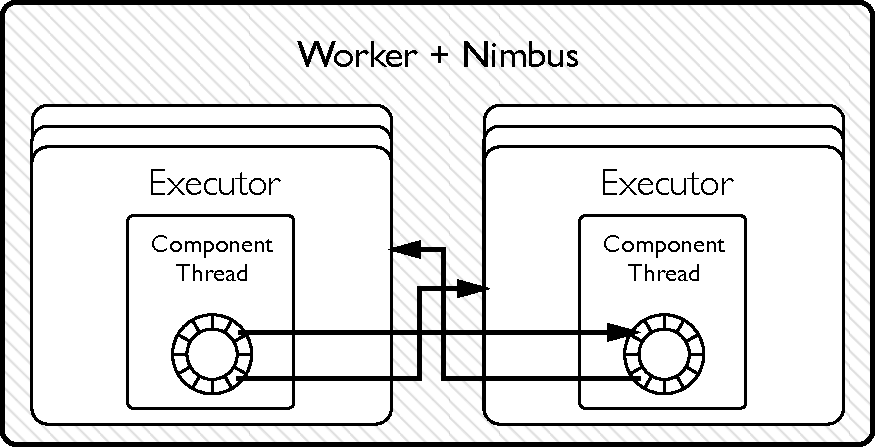
\includegraphics[scale=0.7]{pdf/worker_inside_mc.pdf}
	\caption{Tuple processing in Storm-MC.}
	\label{fig:worker_inside_mc}
\end{figure}

The implementation of tuple processing in Storm-MC can be seen in figure \ref{fig:worker_inside_mc}. As can be seen from the figure, the queues used for remote message sending were stripped away and there is only one Disruptor queue for every executor. Once an executor is done processing a tuple it simply puts it on the Disruptor queue of the bolts downstream.

There were several other options we considered when implementing tuple processing. However, the Disruptor shows superior throughput and latency compared to alternative solutions in \cite{something}.

\todo{find the citation for above claim.}

\section{Differences between Apache Storm and Storm-MC}

\todo{Maybe present this as a table of features.}

%%%%%%%%%%%%%%%%%%%%%%%%%%%%%%%%%%%%%%%%%%%%%
%%
%%				   EVALUATION
%%
%%%%%%%%%%%%%%%%%%%%%%%%%%%%%%%%%%%%%%%%%%%%%


\chapter{Evaluation}

In this chapter we evaluate Storm-MC. We do this by comparing its performance against the local mode of Apache Storm.

\section{Performance}



\section{Challenges}

In this section we are going to discuss challenges we encountered while porting Apache Storm to multi-core machines.


%%%%%%%%%%%%%%%%%%%%%%%%%%%%%%%%%%%%%%%%%%%%%
%%
%%				CONCLUSION
%%
%%%%%%%%%%%%%%%%%%%%%%%%%%%%%%%%%%%%%%%%%%%%%


\chapter{Conclusion}

\section{Future Work}


% use the following and \cite{} as above if you use BibTeX
% otherwise generate bibtem entries
\bibliographystyle{plain}
\bibliography{mybibfile}

\end{document}
